\documentclass[a4paper,11pt]{scrartcl}
\usepackage[ngerman]{babel}
\usepackage[utf8]{inputenc}
\usepackage{tikz}
\usepackage{amsmath}
\usepackage{listings}
\usepackage{url}
\usetikzlibrary{shapes,decorations.pathreplacing,angles,quotes}

\definecolor{dkgreen}{rgb}{0,0.6,0}
\definecolor{gray}{rgb}{0.5,0.5,0.5}
\definecolor{mauve}{rgb}{0.58,0,0.82}

\lstset{frame=tb,
  language=Java,
  aboveskip=3mm,
  belowskip=3mm,
  showstringspaces=false,
  columns=flexible,
  basicstyle={\small\ttfamily},
  numbers=none,
  numberstyle=\tiny\color{gray},
  keywordstyle=\color{blue},
  commentstyle=\color{dkgreen},
  stringstyle=\color{mauve},
  breaklines=true,
  breakatwhitespace=true,
  tabsize=3
}

\begin{document}

\title{Analyzing Big Data Streams}
\author{Florian Kalinke%
  \thanks{E-mail: \texttt{flops.ka@gmail.com}}}
  \date{November 2017}
  \maketitle

  \begin{abstract}
    Das ist die Kurzfassung.
  \end{abstract}

  \tableofcontents

  \section{Einleitung}
  Der Begriff \textit{Big Data} ist eines der aktuellen Buzzwords der Informatik.
  Unternehmen speichern ihre Daten ab und versuchen Erkenntnisse aus dem
  Datenbestand abzuleiten. Abhängig von diesen Ergebnissen können strategische
  Entscheidungen getroffen werden, um dem Unternehmen so einen wirtschaftlichen
  Vorteil zu ermöglichen. Historisch gesehen ist dieses Vorgehen bereits
  etabliert - die zu analysierende Datenmenge steigt allerdings stark an und
  schafft so neue Herausforderungen bei der Analyse der
  Daten.\cite[S.~1]{freiknecht2014}

  Obwohl nicht genau definiert ist, ab wann es sich bei der Datenverarbeitung um
  \textit{Big Data} handelt, hat sich die folgende Definition durchgesetzt:

  Datenmengen, die zu groß, zu komplex oder zu schnelllebig sind, um sie mit
  traditionellen Methoden der Datenhaltung zu speichern und auszuwerten werden
  als Big Data bezeichnet. Diese Einordnung geht davon aus, dass die Daten einem
  oder mehreren der 3 „V“s entsprechen:\footnote{frei übersetzt nach Hilbert,
  M. (2012)}
  \begin{description}
    \item[Volume] Die Datenmengen sind im Tera-, Peta- oder Exabytebereich.
    \item[Velocity] Die Daten müssen in Echtzeit verarbeitet und analysiert
      werden.
    \item[Variety] Die Daten müssen keinem bestimmten Schema entsprechen, sie
      sind sowohl strukturiert, semistrukturiert als auch unstrukturiert.
  \end{description}

  Bei der Verarbeitung der Daten wird zwischen der \textit{Batch-} und
  \textit{Stream-}Verarbeitung differenziert. Die Batch-Verarbeitung geht davon
  aus, dass auf einer begrenzten Menge von Daten operiert wird. Das bedeutet,
  dass die Größe der Daten bekannt und endlich ist. Die Datenmenge kann
  „vollständig“ verarbeitet werden. Im Gegensatz dazu betrachtet die
  Stream-Verarbeitung die Verarbeitung von Daten, die erst während eines
  zeitlichen Verlaufs verfügbar werden.\cite[S.~439]{kleppmann17}

  Betrachtet man exemplarisch die Analyse der Besucherzahlen einer Webseite, so
  lassen sich über Batch-Verarbeitung beispielsweise die Fragen beantworten „Wie
  viele Personen haben die Webseite gestern aufgerufen? Wie viele vorgestern?
  Wie viele in der vergangenen Woche?

  Analog betrachtet die Stream-Verarbeitung die Fragestellungen: Wie viele
  Besucher waren in der letzten Minute auf der Seite aktiv? Wie viele in den
  letzten 10 Sekunden? Sind aktuell Besucher auf der Seite? Über
  Stream-Verarbeitung können diese Daten in Echzeit analysiert und die Ergebnisse
  betrachtet werden.

  Weitere Einsatzgebiete sind zum Beispiel:\cite[S.~465ff.]{kleppmann17}
  \begin{description}
    \item[Fraud Detection] Die Betrugsversuchserkennung versucht plötzliche
      Abweichungen im Nutzungsverhalten einer Kreditkarte zu erkennen und die
      Karte zu sperren, wenn der Verdacht besteht, dass diese gestohlen wurde.
    \item[Fertigungssysteme] Der Zustand von Maschinen in Fabriken soll
      überwacht werden, so dass im Falle eines Fehlverhaltens darauf reagiert
      werden kann.
    \item[High Speed Trading] Abhängig von Schwankungen der Aktien einer Börse
      sollen anhand festgelegter Regeln passende Wertpapiere gekauft oder
      verkauft werden, um den eigenen Gewinn zu maximieren.
    \item[Militärische Überwachung] Die Bewegungen eines potentiellen
      Angreifers werden überwacht, es wird auf auffällige Bewegungsmuster
      reagiert.
    \item[Complex Event Processing] Beim Complex Event Processing wird in einem
      Datenstrom nach vorher festgelegten Mustern gesucht. Das bedeutet der
      Anwender legt Abfragen (ähnlich zu SQL) fest und der Stream wird
      kontinuierlich auf das Auftreten der definierten Muster geprüft.
    \item[Streamanalyse] Die Streamanalyse beschäftigt sich nicht so sehr mit
      besonderen Mustern in den Daten sondern mit analytischen Fragen, zum
      Beispiel wie häufig ein bestimmtes Event aufgetreten ist.
  \end{description}

  Alle Einsatzgebiete haben gemeinsam, dass es sich um „Echtzeitsysteme“ handelt:
  Aus den anfallenden Daten sollen möglichst schnell Informationen gewonnen
  werden. Oft ist es sogar so, dass die Qualität der Informationen, die aus den
  Daten gewonnen werden können, bei längerer Verarbeitungsdauer abnimmt.

  Die vorliegende Arbeit gibt einen allgemeinen Einblick in die Verarbeitung
  von Streams und zeigt im Anschluss detailliert die Möglichkeiten der
  Verarbeitung mit dem Apache Storm Framework. Dazu wird exemplarisch die
  Implementierung einer Software zur Messung der Tippgeschwindigkeit gezeigt.

% TODO Kapitelbeschreibung

  \section{Datenhaltung bei Big Data}
  Die Verarbeitung von den in der Einleitung beschriebenen Datenmengen bringt
  eine Menge an Herausforderungen mit sich: Ein einzelner Rechner ist zu
  schwach, um die Menge an Daten a) abzuspeichern und b) Berechnungen in
  vertretbarer Zeit auf diesen Daten auszuführen. Aus diesem Grund wird für die
  Verarbeitung von Big Data im Normalfall \textit{horizontal} skaliert. Das
  bedeutet, dass die Verarbeitung statt auf einem extrem performanten Rechner
  auf viele „normale“ Rechner verteilt wird.  Hier kommt sogenannte
  \textit{Commodity Hardware} zum Einsatz: Handelsübliche Rechner, die im
  Verbund agieren und auf die anfallende Arbeit aufgeteilt
  wird.\cite[S.~42]{white2010}

  Reduziert man Big Data auf die zu speichernde Datenmenge gibt es drei
  Hauptgründe, die Last auf verschiedene Rechner zu
  verteilen:\cite[S.~145]{kleppmann17}

  \begin{description}
    \item[Skalierbarkeit] Die Daten können aufgrund des Speicherplatzes, der
      Schreibgeschwindigkeit oder der Lesegeschwindigkeit nicht auf einem
      einzelnen Rechner gespeichert werden.
    \item[Fehlertoleranz / Ausfallsicherheit] Das System soll nicht von einer
      einzelnen Maschine abhängig sein. Fällt ein Rechner aus, kann ein anderer
      die Arbeit übernehmen. Je mehr Rechner an einem System beteiligt sind,
      desto wahrscheinlicher ist es, dass einzelne Rechner oder einzelne
      Komponenten ausfallen.
    \item[Latenz] Sind die Daten auf einem Rechner, der sich geographisch nah am
      Ort des Zugriffs befindet, so müssen Netwerkpakete eine geringere Strecke
      zurücklegen und der Zugriff wird beschleunigt.
  \end{description}

  Um Daten verteilt vorzuhalten, gibt es zwei
  Ansätze:\cite[S.~147]{kleppmann17}

  \begin{description}
    \item[Replikation] Die gleichen Daten werden auf verschiedenen Knoten
      vorgehalten, sind also redundant gespeichert. Fällt ein Knoten aus, so
      können die Daten von einem anderen Knoten gelesen werden.
    \item[Partitionierung] Eine große Datenbank wird in Teilmengen zerlegt, die
      dann verschiedenen Knoten zugewiesen werden.
  \end{description}

  Die beiden Ansätze werden in der Praxis häufig kombiniert eingesetzt.

  \section{Das CAP-Theorem}
  Das CAP-Theorem oder \textit{Brewer's Theorem} wurde öffentlich erstmalig im
  Jahr 2000 auf dem \textit{Symposium on Principles of Distributed Computing}
  vorgestellt und im Jahr 2002 formal bewiesen. Das Theorem besagt, dass ein
  verteiltes System nicht mehr als zwei der folgenden drei Garantien bieten
  kann:\cite[S.~51-59]{brewer02}

  \begin{description}
    \item[Konsistenz] Das Lesen eines Wertes liefert immer das Ergebnis des
      letzten Schreibens.
    \item[Verfügbarkeit] Das Lesen eines Wertes liefert immer ein Ergebnis,
      allerdings ohne die Garantie, dass der letzte Schreibvorgang berücksichtigt
      wurde.
    \item[Partitionstoleranz] Das System funktioniert unabhängig von der Zahl der
      verlorenen oder verzögerten Netzwerkpakete.
  \end{description}

  Graphisch wird das CAP-Theorem häufig als Pyramide dargestellt:

% TODO Graphik vom CAP-Theorem

  \section{Lambda Architektur}
  Die Lambda-Architektur wurde 2011 von Nathan Marz im Blogpost „How to beat
  the CAP-Theorem“\cite{marz2011} vorgestellt und beruht auf der Beobachtung,
  dass sich die Komplexität in verteilten Systemen aus dem veränderlichen
  Zustand in Datenbanken („mutable state“) und der Nutzung von inkrementellen
  Algorithmen zur Manipulation dieses Zustands ergibt.  Der Name leitet sich
  aus dem Lambda-Kalkül als Grundlage der funktionalen Programmierung ab:
  Berechnungen im Batch-Layer werden nur auf unveränderlichen Daten ausgeführt.

  Der Autor wirft die Frage auf, wie ein System aussehen würde, dass als
  Kernkomponente eine Append-Only-Datenbank verwendet - das heißt der Zustand
  eines Datums in der Datenbank kann nicht verändert werden. Berechnungen werden
  auf sämtlichen vorhandenen Daten ausgeführt und die Nutzung von inkrementellen
  Algorithmen entfällt.

  $\text{Query} = \text{Function(All Data)}$

  Die Abfrage wird als Batch-Verarbeitung ausgeführt und das Ergebnis
  abgespeichert. Eine Berechnung auf sämtlichen vorhandenen Daten kann sehr lange
  dauern, dass heißt es gibt keine aktuelle Sicht auf die Daten.

  Das Problem wird dadurch gelöst, dass historische Daten über einen Batch-Job
  verarbeitet werden. Neu anfallende Daten verarbeitet der sogenannte Speed- bzw.
  Realtime Layer und dieser füllt so die entstehende Lücke auf. Kombiniert werden
  die beiden Sichten auf die Daten vom \textit{Serving Layer}.

  \begin{figure}[h]
    \center
    \scalebox{.7}{\begin{tikzpicture}[>=stealth]
	\usetikzlibrary{shapes}
	\node (input)			at (3,3) [rounded rectangle, draw, minimum height=1cm,thick] {Input};
	\node (batch)			at (0,0) [cylinder, thick, shape border rotate=90, shape aspect=0.3, draw, minimum height=2.5cm, minimum width=3.5cm] {Batch-Layer};
	\node (serving)		at (0,-3) [rectangle, draw, minimum height=2cm, minimum width=3.5cm,thin] {Serving-Layer};
	\node (speed)			at (6,0) [rectangle, draw, minimum height=2cm, minimum width=3.5cm,thin] {Speed-Layer};
	\node (client)		at (3,-6) [rounded rectangle, draw, minimum height=1cm, minimum width=10cm,thick] {Client};

		\path (input)		edge[->,bend right,dashed,thick] (batch)
		(batch)					edge[->,thick] (serving)
		(serving)				edge[->,dashed,thick] (client)
		(input)					edge[->,bend left,dashed,thick] (speed)
		(speed)					edge[->,dashed,thick] (client);
\end{tikzpicture}
}
    \caption{Schematische Darstellung der Lambda-Architektur}
    \label{fig:lambdaarch}
  \end{figure}

  \subsection{Batch Layer}
  Der Batch-Layer geht davon aus, dass es ok ist, wenn es keine aktuelle Sicht
  auf die Daten gibt und die Berechnungen dadurch entsprechend einfach werden.
  Das heißt der Batch Job läuft, führt seine Berechnungen aus und schreibt das
  Ergebnis in eine Datenbank. Dabei werden schon in der Datenbank bestehende
  Daten vollständig ersetzt. Im Anschluss wird die Neuberechnung angestartet, die
  die in der Zwischenzeit angefallenen Daten mitbetrachtet. Ist diese
  abgeschlossen ersetzt das Ergebnis wieder das vorherige usw.

  \subsection{Speed / Realtime Layer}
  Der Speed-Layer füllt die Versorgungslücke, die entsteht, während die
  Berechnungen des Batch-Layers laufen. Das bedeutet der veränderbare Zusatand,
  der aus der Batch-Verarbeitung heraus gehalten wurde und die damit
  einhergehenden inkrementellen Algorithmen befinden sich jetzt im Speed-Layer
  und führen hier die Berechnungen in Echtzeit aus.

  Die Verschiebung der Komplexität in den Speed-Layer bringt einige Vorteile mit
  sich: Die Daten, die vom Speed-Layer berechnet werden, sind nur so lange
  gültig, wie der Batch-Layer für seine Berechnungen braucht. Das bedeutet ein
  Fehler bei der Datenanalyse kann den Betriebsfluss zwar stören - verschwindet
  aber sobald das Batch-System die Daten in der Datenbank unter Einbeziehung des
  neuen Wertes schreibt.

  An dieser Stelle ist das System auch Fehlern des Entwicklers über toleranter -
  es kann a) ein Fehler bei der Entwicklung der Verarabeitungslogik im
  Batch-Layer programmiert werden, oder b) bei der Entwicklung des Speed-Layers.

  Tritt der Fehler im Batch-Layer auf, so zieht sich der Fehler durch das gesamt
  System und verfälscht die Auswertungen. Da jede Neuberechnung allerdings auf
  sämtlichen historischen Daten basiert (Append-only) kann der Fehler vom
  Entwickler korrigiert werden und die Datenbasis ist nach der Ausbringung der
  Fehlerkorrektur und der nächsten Neuberechnung wieder korrekt. Zukünftige
  Berechnungen des Speed-Layers und Abfragen auf den Datenbestand nutzen die
  korrigiert Version, das heißt es gibt nur temporär eine verfälschte Datenbasis.

  Beim Auftreten eines Fehlers im Speed-Layer, so ist wie oben bereits
  angesprochen, nicht die gesamte Datenbasis vom Fehler beeinflusst, sondern nur
  der Zeitraum, seit die letzte Komplettberechnung des Batch-Layers abgeschlossen
  wurde. Davon ausgehend, dass die Berechnungen auf den Daten im Batch-Layer
  korrekt sind, sind somit die historischen Daten nicht vom Fehler beeinflusst.

  \subsection{Serving Layer}
  Die eigentliche Komplexität der Lambda-Architektur verbirgt sich hinter dem
  \textit{Serving Layer}. Dieser wird im ursprünglichen Artikel von Nathan Marz
  nicht beschrieben und wurde erstmals XXXX genannt. 

  Der Client des verteilten Systems soll im Optimalfall von der Aufteilung der
  Berechnungen in den Batch-Layer und den Speed-Layer nichts mitbekommen. Das
  heißt er muss eine übergreifende Sicht über beide zum Einsatz kommende
  Datenbanken bekommen und Abfragen müssen die Daten aus beiden Datenbanken
  zusammenfassen.

  Die Aufgabe des Serving-Layers ist es, dem Client diese Sicht zur Verfügung zu
  stellen und die Komplexität der Berechnungen im Hintergrund zu verbergen.

  \section{Verarbeitung von Streams}
  Das vorangegangene Kapitel zeigt, dass die Verarbeitung von Batch-Daten der
  Verarbeitung von Streams aufgrund der Komplexität vorzuziehen ist. Beide
  Verfahren können klar voneinander abgegrenzt werden: Bei der Batchverarbeitung
  ist die Größe der Daten bekannt, die Menge der Daten ist endlich und die
  Datenmenge kann „vollständig“ verarbeitet werden.

  Die Streamverarbeitung betrachtet im Gegensatz dazu die Verarbeitung von Daten,
  die erst während eines zeitlichen Verlaufs verfügbar werden. Statt die Daten,
  wie beim klassischen Data-Warehouse, erst zu indizieren und danach Abfragen auf
  den gespeicherten Daten auszuführen, werden die Daten im laufenden Betrieb mit
  statistischen und mathematischen Methoden analysiert.

  Der Betrachter der Ergebnisse erhält so in Echtzeit Rückmeldung über ein
  laufendes System und kann aus den ihm so zur Verfügung gestellten Informationen
  Handlungen ableiten.

  Zusätzlich existiert noch das sogenannte \textit{Micro-Batching}.  Hier wird
  nicht jedes Event / jede Nachricht individuell betrachtet, sondern es werden
  mehrere Nachrichten gesammelt, um dann Berechnungen über diesen kleinen
  Datenbestand auszuführen. Die Zeispanne über welche die Daten zu einem Batch
  zusammengefasst werden nennt sich \textit{Window}.\cite[S.~452]{kleppmann17}
  Im folgenden sind zwei bekannte Windowing-Verfahren vorgestellt, das
  Sliding-Window-Verfahren wird im Praxisteil eingesetzt.

  \subsection{Tumbling Window}
  Ein \textit{Tumbling Window} ist eine Zeitreihe von
  aufeinanderfolgenden und sich nicht überlappenden Intervallen fixer
  Größe.
  \begin{figure}[!h]
    \centering
    \begin{tikzpicture}
       %draw horizontal line   
      \draw[|->, -latex] (0,0) -- (7,0);
      \draw[-, dashed] (-1,0) -- (0,0);

       %draw numbers
      \foreach \x  in {0,...,7} {% 
        \draw (\x,0) node[below=7pt,anchor=north,xshift=0,rotate=0] {\x}; 
        \draw[] (\x,-0.1) -- (\x,0.1);
      }
      % draw braces
      \draw[decoration={brace,mirror,raise=0pt},decorate]
      (0,-1) -- node[below=6pt] {Window 1} (2,-1);
      \draw[decoration={brace,mirror,raise=0pt},decorate]
      (2,-1) -- node[below=6pt] {Window 2} (4,-1);
      \draw[decoration={brace,mirror,raise=0pt},decorate]
      (4,-1) -- node[below=6pt] {Window 3} (6,-1);
    \end{tikzpicture}
    \caption{Schematische Darstellung eines Tumbling Window}
  \end{figure}

  Interpretiert man die im Schaubild dargestellten Intervalle als
  Sekunden, so werden alle Ereignisse von Sekunde 0 bis Sekunde 2
  zusammengefasst, und im Anschluss als Ergebnis geliefert. Im
  Anschluss werden die Ereignisse von Sekunde 2 bis Sekunde 4
  zusammengefasst usw. Das Ergebnis ist immer das des letzten
  abgeschlossenen Intervalls. Jedes Ereignis wird nur einmal
  betrachtet. Das bedeutet, dass jedes Ergebnis maximal 2 Sekunden
  veraltet sein kann.

  \subsection{Sliding Window}
  Ein Sliding Window erzeugt nur ein Ergebnis, wenn in der
  betrachteten Zeit tatsächlich ein Ereignis aufgetreten ist. Die
  Ereignisse können zu mehr als einem Fenster gehören und das Fenster
  wird kontinuierlich um ein bestimmten Wert nach vorne
  geschoben.\cite[S.~472]{kleppmann17}
  \begin{figure}[!h]
    \centering
    \begin{tikzpicture}
       %draw horizontal line   
      \draw[|->, -latex] (0,0) -- (7,0);
      \draw[-, dashed] (-1,0) -- (0,0);

       %draw numbers
      \foreach \x  in {0,...,7} {% 
        \draw (\x,0) node[below=7pt,anchor=north,xshift=0,rotate=0] {\x}; 
        \draw[] (\x,-0.1) -- (\x,0.1);
      }
      % draw braces
      \foreach \x  in {0,...,5} {% 
        \draw[decoration={brace,mirror,raise=0pt},decorate]
        (\x,-\x/3-1) -- node[below=6pt] {} (\x+2,-\x/3-1);
      }
      \draw (6,-3) node {Window $n$};
    \end{tikzpicture}
    \caption{Schematische Darstellung eines Sliding Window}
  \end{figure}

  Im Schaubild ist zu sehen, wie das Betrachtungsfenster mit der Zeit
  wandert, die einzelnen Fenster überschneiden sich. So kann ein
  Ereignis verschiedenen Fenstern zugeordnet werden. Das bedeutet, es
  wird immer eine aktuelle Sicht auf das Ergebnis präsentiert. Auch
  hier muss festgelegt werden, wie häufig das Ergebnis aktualisiert
  werden soll - es gibt also auch eine geringe Latenz.

% TODO Event / Nachricht definieren

% TODO Wo kommen diese Informationen her? Message Broker: AMQP/JMS-Style Broker
% vs. Log-Based-Message Broker

% TODO Wieso diese Frameworks? => Open Source, können problemlos verprobt
% werden

% TODO Avro / Serialisierung von Nachrichten

  \section{Apache Storm}

  Apache Storm bezeichnet eine von der Apache Software Foundation
  bereitgestellte kostenlose Open-Source Software. Dieses Framework
  erlaubt die Echtzeitverarbeitung von unbegrenzten Datenströmen und
  erreicht dabei einen Durchsatz von bis zu einer Million Tuple pro
  Sekunde pro Knoten des verteilten Systems. Das Framework wird auf
  der zugehörigen Website als skalierbar und fehlertolerant beworben.
  Zudem bietet es ein sogenanntes Guaranteed-Message-Processing, d.h.
  das Framework gewährleistet, dass Nachrichten auf jeden Fall
  verarbeitet werden und nicht verloren gehen.\cite{apachestorm}

  \subsection{Storm Komponenten}

  Der Einsatz des Storm Frameworks setzt die Kenntnis einiger
  Begrifflichkeiten voraus. Diese werden im Folgenden kurz eingeführt
  und erläutert.\cite[S.~53ff.]{stormpresentation2011}

  \paragraph{Tuple}
  Ein Tuple bezeichnet im Kontext des Frameworks eine Nachricht, die
  von diesem verarbeitet wird. Mathematisch ist ein Tupel allgemein wie folgt
  definiert:
  \begin{quote}
    Ein Tupel besteht aus einer Liste endlich vieler, nicht
    notwendigerweise voneinander verschiedener Objekte.
  \end{quote}
  %\setlength{\abovedisplayskip}{-20pt}
  %\setlength{\abovedisplayshortskip}{-20pt}

  \begin{align*}
    (x_1, \ldots , x_n)
  \end{align*}

  \paragraph{Stream}
  Ein Stream fasst mehrere Tupel zu einem Datenstrom zusammen. Storm
  vearbeitet diese Streams.
  \begin{quote}
    [\ldots] einen kontinuierlichen Fluss von Datensätzen, dessen Ende
    meist nicht im Voraus abzusehen ist; die Datensätze werden
    fortlaufend verarbeitet, sobald jeweils ein neuer Datensatz
    eingetroffen ist.
  \end{quote}

  \begin{align*}
    (x_1, \ldots , x_n)
    (x_1, \ldots , x_n)
    (x_1, \ldots , x_n)
    (x_1, \ldots , x_n)
  \end{align*}
  \begin{figure}[!h]
    \centering
    \vspace*{-1cm}
    \begin{tikzpicture}
       %draw horizontal line   
      \draw[|->, -latex] (0,0) -- (7,0);
    \end{tikzpicture}
  \end{figure}

  \paragraph{Spout}
  Ein Spout, dt. „die Quelle“, erzeugt den zu verarbeitenden Stream.
  Quellen können verschiedene angebundene Systeme sein, zum
  Beispiel Message Queuing Systeme (Apache Kafka, Twitter Kestrel),
  Datenbanksysteme (Redis) oder Web-Ressourcen (Twitter).

  Storm stellt für die genannten Systeme bereits fertige Spouts zur
  Verfügung. Ein Spout ist sowohl für das Erzeugen neuer Nachrichten,
  als auch für das Verarbeiten der Rückmeldung, dass eine Nachricht
  erfolgreich verarbeitet wurde, zuständig. Analog dazu muss der Spout
  auch verloren gegangene Nachrichten neu senden. Dadurch wird das
  Guaranteed-Message-Processing möglich.

  % TODO Wie funktioniert das GMP?

  \paragraph{Bolt}
  Die eigentliche Verabeitungslogik für die Streamverarbeitung mit
  Storm wird in sogenannten Bolts realisiert. Der Bolt hat dazu eine
  \textit{execute(\ldots)}-Methode, diese wird vom Framework für jedes
  Tupel einzeln aufgerufen. Das Framework setzt die beiden Parameter
  \textit{input} und \textit{collector}. \textit{Input} ist das zu
  verarbeitende Tupel und über den \textit{collector} kann die
  Nachricht an einen anderen Bolt weitergegeben werden. Die
  Kombination verschiedener Spouts und Bolts ist im Folgenden Kapitel
  beschrieben.

  \begin{lstlisting}[caption={Methodensignatur einer Bolt-Implementierung}]
  void execute(Tuple input, BasicOutputCollector collector)
  {
    /* do some magic stuff here, e.g:
    * - count words
    * - write to database
    * - combine data
    */
    ...
  }
  \end{lstlisting}

  In der \textit{execute}-Methode kann der Entwickler unabhängig vom
  Framework die Anwendungslogik realisieren. Hier ist zu beachten,
  dass der die Bolt-Klasse vor der Nutzung serialisiert und auf die
  Knoten des verteilten Systems transferiert wird: Es ist daher nicht
  möglich im Konstrukter nicht serialisierbare Objekte zu instantieren.
  Werden solche benötigt, so muss die Instantierung in der
  \textit{prepare(\ldots)}-Methode erfolgen. Diese wird auch vom
  Framework aufgerufen.

  \paragraph{Topologie}
  Die \textit{Topologie} bezeichnet den Zusammenschluss verschieder
  Spouts und Bolts in ein Gesamtkonstrukt von welchem die Streams
  verarbeitet werden. Spouts können dabei ihre Nachrichten an ein oder
  mehrere Bolts senden und diese können äquivalent neue Nachrichten
  erzeugen und weitergeben oder erhaltene Nachrichten als letzter
  Knoten des Graphs abschließend verarbeiten.

  \begin{figure}[!h]
    \center
    \scalebox{.7}{\begin{tikzpicture}[>=stealth]
	\usetikzlibrary{shapes}
	\node (spout0)			at (0,2.5) [rounded rectangle, draw, minimum height=1cm,thick] {Spout};
	\node (spout1)			at (0,-2) [rounded rectangle, draw, minimum height=1cm,thick] {Spout};

	\node (bolt0)			at (3,4) [rectangle, draw, minimum height=1cm,thick] {Bolt};
	\node (bolt1)			at (3,1) [rectangle, draw, minimum height=1cm,thick] {Bolt};
	\node (bolt2)			at (3,-2) [rectangle, draw, minimum height=1cm,thick] {Bolt};

	\node (bolt3)			at (6,2.5) [rectangle, draw, minimum height=1cm,thick] {Bolt};


	\path (spout0)		edge[->,thick] (bolt0)
		(spout0)				edge[->,thick] (bolt1)
		(spout0)				edge[->,thick] (bolt2)
		(spout1)				edge[->,thick] (bolt2)
		(bolt0)	  			edge[->,thick] (bolt3)
		(bolt1)	  			edge[->,thick] (bolt3);
\end{tikzpicture}
}
    \caption{Schematischer Aufbau einer Storm-Topologie}
    \label{fig:topology}
  \end{figure}

  Im Schaubild sind zwei Spouts dargestellt, die die Nachrichten an
  drei beziehungsweise einen Bolt weitergeben. Innerhalb der Bolts
  findet eine Verarbeitung statt, bevor eine neue Nachricht an den
  hinteren Bolt gesendet wird. Hier ist zum Beispiel denkbar, dass
  Ergebnisse in einer Datenbank persistiert werden.

  \subsection{Guaranteed-Message-Processing}
  Die Verantwortung, dass Nachrichten nicht verworfen werden, bevor
  diese vollständig verarbeitet sind liegt beim Sender der Nachricht,
  das heißt, dass der Spout überwachen muss welche der von ihm
  gesendeten Nachrichten fertig verarbeitet wurden. Während der
  verschiedenen Verarbeitungsschritte innerhalb der Topologie bildet
  sich ein sogenannter „Tupel-Baum“. Es wird nicht immer das gleiche
  Tupel verarbeitet, sondern die jeweiligen Bolts erzeugen ein neues
  Tupel, welches auf dem Empfangenen basiert. Schlägt die Verarbeitung
  eines dieser Tupel fehl, so muss das Ursprungstupel noch einmal
  gesendet werden.\cite{stormguaranteedprocessing}

  \paragraph{At-least-once-Semantik}
  Das im vorhergehenden Paragraphen beschriebene Vorgehen stellt
  sicher, dass eine Nachricht mindestens einmal korrekt verarbeitet
  wird. Der Ausfall eines Knotens beziehungsweise ein technischer
  Fehler kann dafür Sorgen, dass ein Tupel nicht vollständig
  verarbeitet wird und damit neu gesendet wird. Haben basierend auf
  diesem Tupel bereits Berechnungen stattgefunden, die an einer Stelle
  persistiert wurden, so wird nun unter Umständen das Ergebnis
  verfälscht. Storm garantiert hier, dass die Nachricht auf jeden Fall
  einmal verarbeitet wird - im Fehlerfall kann es aber vorkommen, dass
  die Nachricht mehrfach verarbeitet wird.

  \paragraph{Exactly-once-Semantik}
  In bestimmten Szenarien soll sichergestellt sein, dass Nachrichten
  auch im Fehlerfall nur genau einmal (\textit{exactly-once})
  verarbeitet werden und die darauf ausgeführten Berechnungen damit
  unabhängig von eventuellen Ausfällen oder auftretenden Fehlern sind.
  Die Exactly-Once-Semantik gewährleistet dies. Eine entsprechende 

  \subsection{Apache Storm Trident} 
  Soll mit Storm eine Exactly-Once-Verarbeitung realisiert werden,
  kann dafür das Apache Storm Trident Framework genutzt werden. Statt
  wie in regulären Bolts jedes Tupel einzeln zu verarbeiten werden
  hier verschiedene Tupel zu sogenannten Micro-Batches
  zusammengefasst. Die Reihenfolge der Verarbeitung der Micro-Batches
  ist strikt sortiert, das heißt es wird erst ein Batch fertig
  verarbeitet, bevor mit der Verarbeitung des folgenden Batches
  angefangen wird.\cite{stormtrident}

  Trident bringt für die Verarbeitung der Streams vorgefertigte
  Operationen mit. Es können Merges und Joins, Aggregationen,
  Gruppierungen, Funktionen und Filter auf die jeweiligen Stream
  angewendet werden.

  Die Exactly-Once-Verarbeitung kann durch den Spout konfiguriert
  werden. Erreicht wird dies durch das Mitführen von State, wenn Daten
  aggregiert werden. Unterschieden wird zwischen den
  Folgenden:\cite{stormtridentstate}

  \begin{description}
    \item[Transactional] In jedem erneut gesendeten Batch sind genau
      die Tupel, die vorher auch im Batch waren. Fällt ein Teil des
      Zuliefersystems aus, zum Beispiel Apache Kafka, kann nicht
      weitergearbeitet werden, da der passende Batch nicht wieder
      geschickt werden kann.

      Bei der Speicherung von Werten wird neben dem eigentlichen Wert
      zusätzlich die ID des Batches gespeichert, der diese Änderung
      ausgelöst hat. Da die Batches sortiert sind (die ID steigt immer
      an) lässt sich so vor der Änderung eines Wertes feststellen, ob
      dieser bereits für den akutellen Batch angepasst wurde oder ob
      der Batch neuer ist.
    \item[Opaque Transactional]
      Dieser Spout gewährleistet, dass jedes Tupel in genau einem
      Batch erfolgreich verarbeitet wird und trifft keine Aussage über
      die Beschaffenheit der Batches. Das bedeutet, dass das
      Fehlschlagen der Verarbeitung eines Tupels dazu führt, dass das
      Tupel im Anschluss in einem anderen Batch nochmal geschickt
      wird.

      Da nun keine Aussage mehr über eine bereits stattgefundene
      Verarbeitung über die Batch-ID getroffen werden kann muss
      zusätzlich ein weiterer Zustand gespeichert werden. Neben dem
      eigentlichen Wert wird daher auch der vorherige Wert und die
      Transaktions-ID gespeichert.
    \item[Non-Transactional]
      Diese Art von Spout trifft keine Aussagen über die Inhalte eines
      Batches. Das bedeutet es kann sowohl eine At-Most-Once-Semantik
      (Fehler werden ignoriert, Tupel gehen verloren) als aus
      At-Least-Once-Sematik erreicht werden. Eine
      Exactly-Once-Verarbeitung ist nicht möglich.
  \end{description}

  \section{Echtzeitanalyse von Tastatureingaben}
  Die vorgestellten Konzepte und der Einsatz des Apache Storm
  Frameworks soll anhand eines kleinen Beispiels praktisch illustriert
  werden.

  Das klassische Beispiel für die Demonstration der Big Data
  Verarbeitung ist der \textit{Word Count}. Hier wird in einer oder
  mehreren Textdateien die Häufigkeit des Vorkommens jedes Wortes
  gezählt. Mittlerweile gilt dieses Beispiel als das \textit{Hello
  World} von Big Data.

  Dieses Beispiel erfordert keine Echtzeitverarbeitung und ist somit
  für die Verprobung der Stream Verarbeitung nicht geeignet. Statt die
  Wörter statisch aus einer Textdatei zu verarbeiten werden die Wörter
  daher vom Nutzer entsprechend der Aufforderung eingegeben, um die
  Tippgeschwindigkeit des Anwenders festzustellen.

  \begin{figure}[!h]
    \centering
    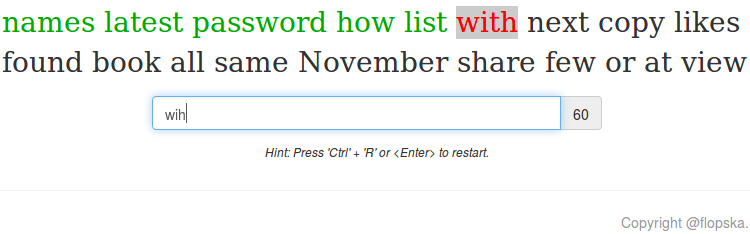
\includegraphics[scale=0.4,natwidth=750,natheight=234]{../presentation/img/webapp.png}
    \caption{Erzeugen eines Wort-Streams\protect\footnotemark}
  \end{figure}

  \footnotetext{Screenshot von \url{http://github.com/flopska/bigdatatools/}}

  Die Eingabe erfolgt über eine in HTML und JavaScript geschriebene
  WebApp. Diese präsentiert dem Nutzer eine Liste von Wörtern und
  darunter ein Eingabefeld in welches das aktuell hervorgehobene Wort
  eingegeben werden soll. Schreibt der Nutzer das Wort richtig, so
  färbt es sich grün. Bei einem Fehler wird das Wort rot dargestellt.
  Das Betätigen der Leertaste bewegt die Hervorhebung zum nächsten
  Wort und löscht den Inhalt des Eingabefeldes.

  Jedes korrekt eingegebene Wort wird über einen Ajax-Aufruf an eine
  REST-Schnittstelle geschickt und dann serverseitig weiter
  verarbeitet.

  \begin{figure}[!h]
    \center
    \scalebox{.7}{\begin{tikzpicture}[>=stealth]
	\usetikzlibrary{shapes}
  \node (webapp)			at (0,2) [rectangle, draw, minimum height=1cm,thick,align=center] {Typing Webapp \\ {[.js]}};
  \node (kafka)			at (6,0) [rectangle split, rectangle split parts=8, rectangle split horizontal, draw, minimum height=1cm,thick,align=center,label=below:Kafka Message Queue] {};
  \node (kafka-rest)			at (6,2) [rectangle, draw, minimum height=1cm,thick] {kafka-rest};
  \node (confluent)			at (6,1) [rectangle, draw, minimum height=4.5cm,thick,text width=6cm,align=center,label=below:confluent] {};
  \node (storm)			at (12,0) [rectangle, draw, minimum height=1cm,thick,align=center] {Storm Topology\\ {[.java]}};

		\path
		(webapp)					edge[->,thick] (kafka-rest)
		(kafka-rest)					edge[->,thick] (kafka)
		(kafka)					edge[->,thick] (storm);
\end{tikzpicture}
}
    \caption{Architektur des Word Count Beispiels}
    \label{fig:wordcountsamplearchitecture}
  \end{figure}

  Die REST-Schnittstelle nimmt die Nachricht entgegen und schreibt
  diese in einen Kafka-Topic. Von dort wird die Nachricht von Storm
  weiter verarbeitet. Diese Architektur ist im obigen Schaubild
  schematisch dargestellt.

  Die Schnittstelle wurde nichts selbst entwickelt, sondern hier kommt
  die Schnittstelle aus der \textit{confluent}-Distribution zum
  Einsatz.

  % TODO Wieso confluent?

  Da jede Nachricht nur ein einziges Mal verarbeitet werden soll, wird
  für die tatsächliche Verarbeitung Storm Trident eingesetzt. Für ein
  Sliding Window mit der Länge von 10 Sekunden wird die Zahl der
  eingegebenen Wörter gezählt. Aktualisiert wird der ausgegebene
  Zähler jede Sekunde.

  \begin{lstlisting}[caption={Beispielimplementierung zur Ermittlung der Tippgeschwindigkeit}]
  public static void main(String[] args) {
    TridentTopology topology = new TridentTopology();
    BrokerHosts zk = new ZkHosts("localhost");
    TridentKafkaConfig spoutConf = new TridentKafkaConfig(zk, "words");
    spoutConf.scheme = new SchemeAsMultiScheme(new StringScheme());
    OpaqueTridentKafkaSpout spout = new OpaqueTridentKafkaSpout(spoutConf);
    WindowsStoreFactory mapState = new InMemoryWindowsStoreFactory();

    SlidingDurationWindow windowConfig = SlidingDurationWindow.of(
    new BaseWindowedBolt.Duration(10, TimeUnit.SECONDS),
    new BaseWindowedBolt.Duration(1, TimeUnit.SECONDS));
    topology.newStream("words", spout)
    .window(windowConfig, mapState, new Fields("str"), new CountAsAggregator(), new Fields("count"))
    .filter(new Debug());

    LocalCluster cluster = new LocalCluster("localhost", 2181L);
    cluster.submitTopology("localCluster2", new Config(), topology.build());
  }
  \end{lstlisting}

  % TODO Zeitbetrachtung : Es wird die Serverzeit genutzt

  \section{Zusammenfassung / Fazit}
  \bibliography{bib}
  \bibliographystyle{alpha}


  \end{document}
